\documentclass[11pt,spanish,a4paper]{article}
% Versión 2.o cuat 2015 Víctor Bettachini < bettachini@df.uba.ar >

\usepackage{babel}
\addto\shorthandsspanish{\spanishdeactivate{~<>}}
\usepackage[utf8]{inputenc}
\usepackage{float}

\usepackage{units}
\usepackage[separate-uncertainty=true, multi-part-units=single, locale=FR]{siunitx}

\usepackage{amsmath}
\usepackage{amstext}
\usepackage{amssymb}

\newcommand{\pvec}[1]{\vec{#1}\mkern2mu\vphantom{#1}}

% \usepackage{tikz}
% \input{DimLinesTikz}
% \usetikzlibrary{decorations.pathmorphing, patterns}

\usepackage{graphicx}
\graphicspath{{./graphs/}}

\usepackage[margin=1.3cm,nohead]{geometry}
% \voffset-3.5cm
% \hoffset-3cm
% \setlength{\textwidth}{17.5cm}
% \setlength{\textheight}{27cm}

\usepackage{lastpage}
\usepackage{fancyhdr}
\pagestyle{fancyplain}
\fancyhead{}
\fancyfoot{{\tiny \textcopyright Departamento de Física, FCEyN, UBA}}
\fancyfoot[C]{ {\tiny Actualizado al \today} }
\fancyfoot[RO, LE]{Pág. \thepage/\pageref{LastPage}}
\renewcommand{\headrulewidth}{0pt}
\renewcommand{\footrulewidth}{0pt}

% \def \materia {Física II para químicos}
\def \periodo {cuatrimestre de verano - 2017}
\def \website {http://materias.df.uba.ar/f2qa2017v}


\begin{document}
\noindent
\textbf{Física II (Químicos)}\hfill \textcopyright {\tt DF, FCEyN, UBA}
% \textbf{\materia}\hfill \periodo
\begin{center}
  \textsc{\large Guía 3: Corriente eléctrica - Ley de Ohm - Leyes de Kirchoff - Conexión de resistencias - Teorema de Thévenin} 
\par\end{center}{\large \par}


\begin{enumerate}
% \begin{description}

\section*{Corriente eléctrica - Ley de Ohm}

  \item Un alambre de cobre de \SI{2}{\milli\metre} de radio y \SI{1}{\metre} de longitud se estira hasta cuadruplicar su longitud (las secciones inicial y final son uniformes).
  % \item[Problema 1] Un cable de cobre (resistividad del Cu: \SI{1.7E-8}{\ohm\metre}) de \SI{2}{\milli\metre} de radio y \SI{1}{\metre} de longitud se estira hasta cuadruplicar su longitud (las secciones inicial y final son uniformes).
Resistividad del cobre, \(\rho_{\mathrm{Cu}}= \SI{1.7E-8}{\ohm\metre}\).
\begin{enumerate}
  \item Calcular la resistencia antes y después del estiramiento, suponiendo que la resistividad no varía.
  \item Por el cable de cobre de \SI{2}{\milli\metre\squared} de sección circula una corriente de \SI{1}{\ampere}.
Si hay un electrón de conducción por cada átomo, encuentre la velocidad media de los electrones.
Datos: \(\mathrm{\delta_{Cu}} = \SI{9}{\gram\per\centi\metre\cubed}\), \(\mathrm{e} = \SI{1.60E-19}{\coulomb}\), \(\mathrm{N_A} = \SI{6E23}{\per\mol}\), \(\mathrm{A_{Cu}}= 63.5\).
  \item Calcular la resistencia eléctrica de una plancha, una estufa de cuarzo, una lamparita eléctrica de \SI{60}{\watt} y una lamparita de linterna.
\end{enumerate}
 
 
\section*{Leyes de Kirchoff - Conexiones de resistencias}

	\item \begin{minipage}[t]{0.7\textwidth}
	% \item \begin{minipage}[t][3cm]{0.7\textwidth}
		Para el circuito representado en la figura:
		\begin{enumerate}
			\item Calcular las corrientes de ramas y de mallas.
			\item Repetir después de cambiar una de las resistencias de \SI{12}{\ohm} por una de \SI{6}{\ohm}. 
		\end{enumerate}
    \end{minipage}
    \begin{minipage}[c][1em][t]{0.2\textwidth}
            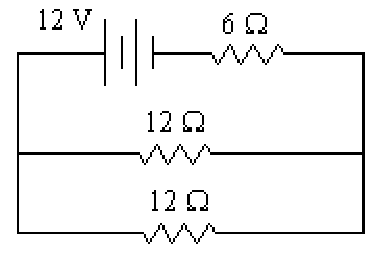
\includegraphics[width=\textwidth]{p3e02}
    \end{minipage}


	\item \begin{minipage}[t]{0.6\textwidth}
		Para el circuito que muestra la figura, calcular:
		\begin{enumerate}
			\item las corrientes \(i_1\) e \(i_2\),
			\item la diferencia de potencial entre los puntos C y D,
			\item y la potencia disipada por las resistencias de \SI{5}{\ohm}.
			\item De colocarse un amperímetro en serie con la batería de \SI{20}{\volt}, ¿qué corriente mide si la resistencia interna del amperímetro es \(R_a = \SI{1}{\ohm}\)?
			\item Repita el punto anterior pero ahora considerando que el amperímetro está en serie con la resistencia de \SI{3}{\ohm}.
			\item Comparar los dos puntos anteriores con el primero.
		\end{enumerate}
    \end{minipage}
    \begin{minipage}[c][1em][t]{0.35\textwidth}
            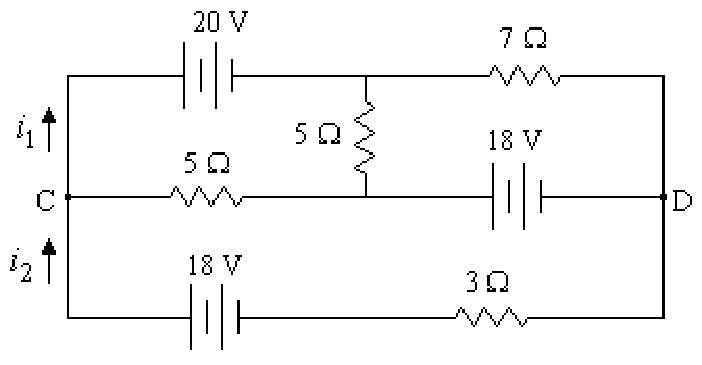
\includegraphics[width=\textwidth]{p3e03}
    \end{minipage}

\item Obtener las corrientes en cada rama.

    \begin{center}
    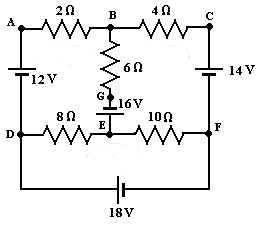
\includegraphics[width=0.45 \textwidth]{kirchhoff}
    \end{center}


\item
    En este caso luego de calcular las corrientes en cada rama calcular la que pasa por \(R_3\) si \(R_2=\SI{125}{\ohm}\).

    \begin{center}
    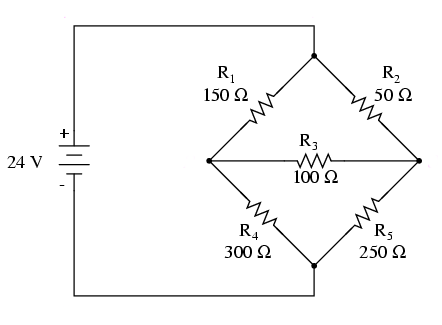
\includegraphics[width=0.5 \textwidth]{wheatstone}
    \end{center}


\item \textbf{Ejercicio opcional.} Obtener las corrientes en cada rama.

    \begin{center}
    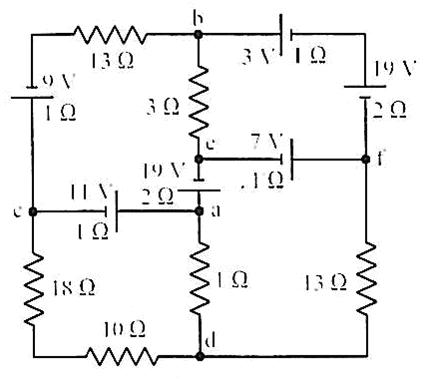
\includegraphics[width=0.45 \textwidth]{Circuitos_electricos_3}
    \end{center}



\section*{Teorema de Thévenin}

	\item \begin{minipage}[t][3.5cm]{0.6\textwidth}
		En el circuito de la figura calcular:
		\begin{enumerate}
			\item la resistencia equivalente vista desde la fuente,
			\item la corriente \(i\) y la caída de potencial entre los puntos B y C,
  			\item y la potencia entregada por la fuente.
		\end{enumerate}
    \end{minipage}
    \begin{minipage}[c][1em][t]{0.3\textwidth}
            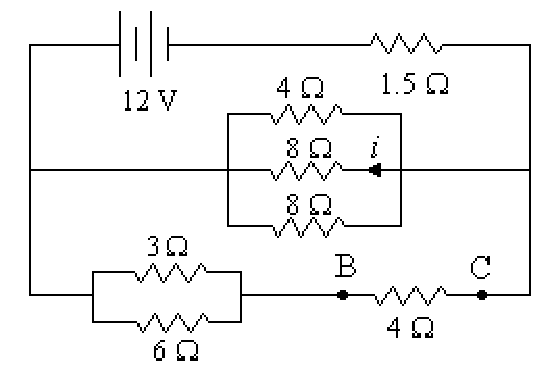
\includegraphics[width=\textwidth]{p3e04}
    \end{minipage}


	\item \begin{minipage}[t][4.5cm]{0.6\textwidth}
		Determinar la potencia suministrada a una resistencia que se conecta entre A y B si su valor es:
		\begin{enumerate}
			\item \(R_1= \SI{1}{\ohm}\),
			\item \(R_2= \SI{5}{\ohm}\),
			\item \(R_3= \SI{10}{\ohm}\),
			\item o \(R_4\) tal que la transferencia de potencia resulte máxima.
		\end{enumerate}
    \end{minipage}
    \begin{minipage}[c][1em][t]{0.35\textwidth}
            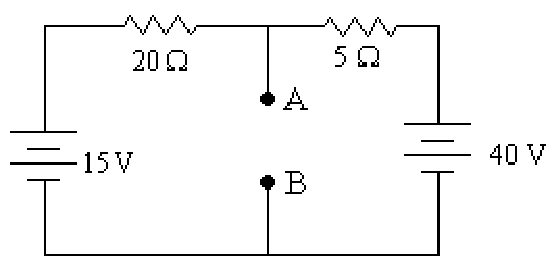
\includegraphics[width=\textwidth]{p3e05}
    \end{minipage}



	\item \begin{minipage}[t][4.5cm]{0.6\textwidth}
% \item \setlength{\parskip}{0cm}
	\begin{enumerate}
		\item Obtener el circuito equivalente de Thévenin para el puente de la figura (conocido como puente de Wheatstone) visto desde los puntos A y B.
		\item Entre A y B se conecta una resistencia \(R\).
			Calcular la corriente que circula por ella en función de \(\varepsilon\), \(R_1\), \(R_2\), \(R_ 3\), \(R_4\) y \(R\).
		\item Determine la relación entre las resistencias para la cual la corriente que circula por el amperímetro es nula.
			Ésta se llama condición de equilibrio del puente y se emplea para medir resistencias con precisión.
		\item Hallar la potencia disipada por \(R\) cuando: \(\varepsilon= \SI{1}{\volt}\), \(R_4= \SI{1.1}{\ohm}\), \(R_1= R_2= R_3= \SI{1}{\ohm}\), y \(R= \SI{0.1}{\ohm}\).
	\end{enumerate}
    \end{minipage}
    \begin{minipage}[c][1em][t]{0.35\textwidth}
            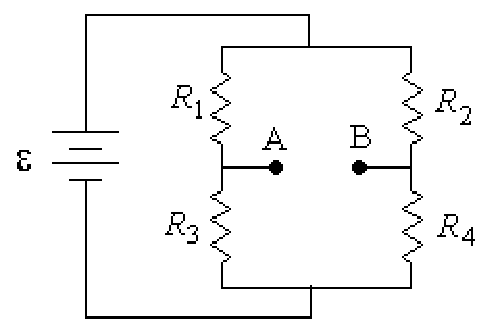
\includegraphics[width=\textwidth]{p3e06}
    \end{minipage}





\end{enumerate}
% \end{description}
\end{document}
